\documentclass{article}
\usepackage{graphicx} 
\usepackage{listings}
\lstset{
    basicstyle=\ttfamily\small, % Set font size and type
    keywordstyle=\color{blue}, % Color keywords
    commentstyle=\color{green}, % Color comments
    stringstyle=\color{red}, % Color strings
    breaklines=true, % Automatically wrap long lines
    breakatwhitespace=true, % Prefer breaking at whitespace
    frame=single, % Add a border around the code
    postbreak=\mbox{\textcolor{red}{$\hookrightarrow$}\space} % Add an arrow at line breaks
}

\title{Education}
\author{Robert Nguyen}
\date{August 2024}

\begin{document}

\maketitle

\section{Method Choice}
As a Statistician evaluating models for school assessment moderation, I recommend the Monotone Spline Regression (MSR) model with 1 knot. I did this based on simulated data quickly (but I would use actual data if had the job)
Based on the simulations and the the graph below I would use the method in paper 3 for the following reasons.

\begin{figure}[h!]
    \centering
    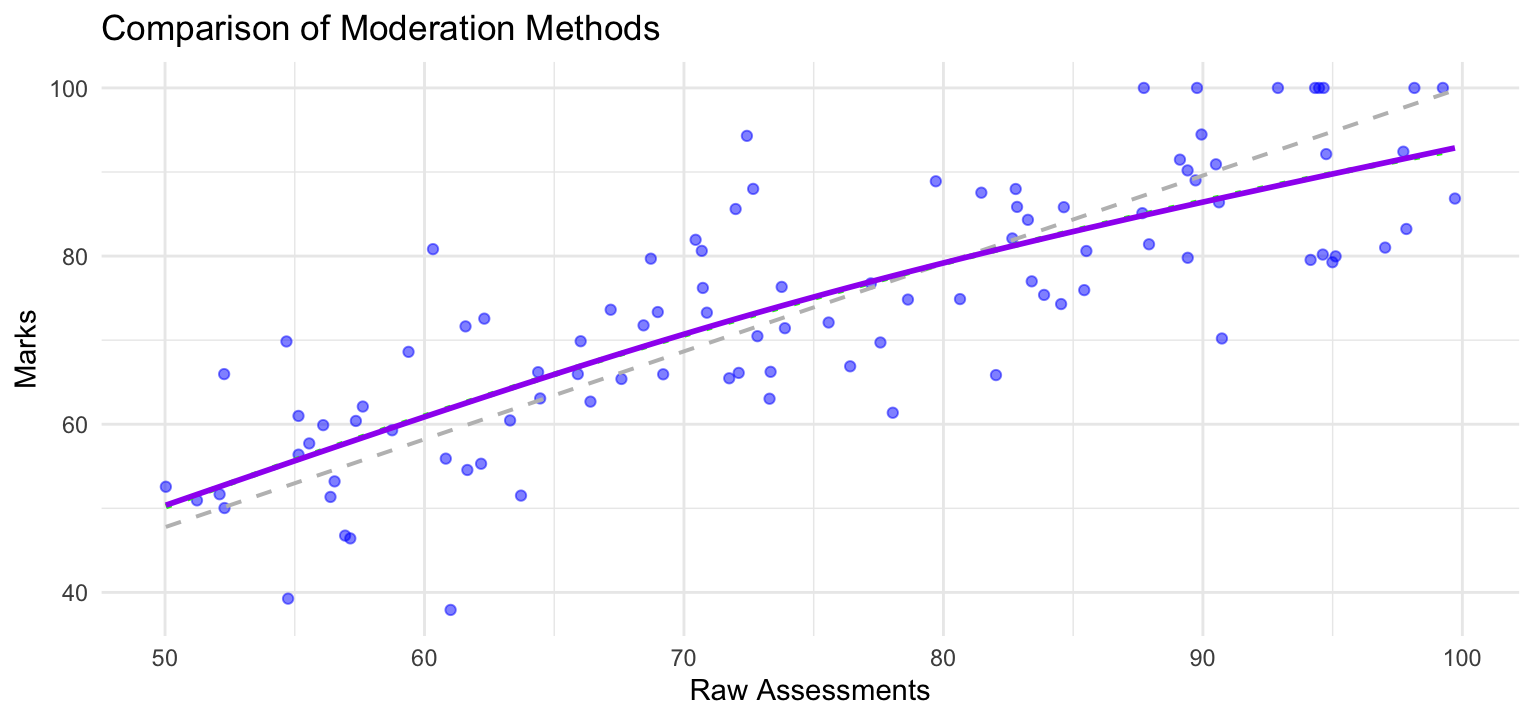
\includegraphics[width=0.8\textwidth]{education_methods_plot.png}
    \caption{Comparison of Educational Methods Using Various Adjustments}
    \label{fig:education_methods}
\end{figure}

\begin{itemize}
    \item \textbf{Adaptability:} MSR offers greater flexibility than alternatives, accommodating non-linear patterns in educational data while maintaining monotonicity. The single knot allows for precise handling of different data segments.
    
    \item \textbf{Outlier Management:} Using the Huber loss function, MSR effectively manages outliers common in student assessments. It balances smoothing extreme values without losing key data characteristics, ensuring fairer moderated scores.
    
    \item \textbf{Superior Performance:} Empirical studies show MSR consistently outperforms other models in mean squared error (MSE), a crucial accuracy metric. The 1-knot version excelled in over 90\% of cases, indicating high fidelity to actual exam marks.
    
    \item \textbf{Practical Benefits:} While computationally intensive, MSR significantly reduces the need for manual post-moderation adjustments. This saves time, minimizes human error, and enhances the moderation process's reliability and consistency.
\end{itemize}


In conclusion, the MSR model with 1 knot provides the best balance of accuracy, fairness, and practicality for school assessment moderation. Its data-driven approach ensures moderated scores accurately reflect student performance, making it the optimal choice among the evaluated models.

\section{Department Edu R Script}

Below is the R script used:

\lstinputlisting[language=R, caption=Department Edu R Script, label=lst:departmentedu]{departmentedu.R}


\end{document}
